\section{Discussion}



% \subsubsection{Method Comparison}

\begin{table}[t]
\centering
\caption{Average method rank~($\downarrow$) for \benchmarkname tasks~(c.p. stands for change points). Top results are shown in \first{first}, \second{second}, \third{third}.} \label{tab:overall}
\resizebox{\linewidth}{!}{%
\begin{tabular}{l l |ccccc|c|cccc}
\toprule
 %\multirow{2}{*}{ %\diagbox{Name}{Data} 
 % \begin{tabular}{l}
 %      \hspace*{0.75cm}Dataset \\
 %      Models
 % \end{tabular}

 %  \begin{tabular}{l}
 %      Models
 % \end{tabular}
 %} 
&& \multicolumn{5}{c|}{Periodicity} & Cause \& & \multicolumn{4}{c}{Spatio-temporal long-range} \\
& Method & \multicolumn{2}{c}{$\Pdet{2,n}$} &\multirow{2}{*}{$\Pdet{k,1}$} & \multicolumn{2}{c|}{$\Psto{2,n}$} & Effect &  \multicolumn{4}{|c}{$\longrange{\lag,d}$} \\    
& & all $t$  & c.p. &  & $p=0.5$ & $p=0.9$ & $\causeeffect{\ell}$ & $\lag\!=\!1$ & $\lag\!=\!4$ & $\lag\!=\!16$ & $\lag\!=\!32$ \\ 
%
%
%  & \multirow{2}{*}{Method}& \multicolumn{5}{c|}{Periodicity} & \multicolumn{1}{c|}{
% \begin{tabular}{@{}c@{}}Cause \& \\ Effect\end{tabular}
% } & \multicolumn{4}{c}{Spatio-temporal long-range} \\   
%     & & $(2, n)$ - A & $(2, n)$ - C & $(k, 1)$ & $(0.5)$ & $(0.9)$ & $\causeeffect{\ell}$ & $(1, d)$ & $(4, d)$ & $(16, d)$ & $(32, d)$ \\ 
  \midrule

  \multirow{4}{*}{\rotatebox[origin=c]{90}{CTDG}} & 
  CTAN & 5.625 & \third{3.75} & 7.625 & \second{3.167} & 5.167 & 6.4 & 10.0 & 8.6 & 8.4 & 6.8 \\
  & DyGFormer & \second{3.25} & \second{3.5} & \third{2.625} & 7.167 & 7.5 & \third{3.2} & \second{2.2} & \second{1.8} & \third{3.0} & \second{3.4} \\
  & TGAT & 4.75 & 5.0 & 4.375 & \third{3.667} & \second{3.167} & \second{2.6} & 3.8 & \first{1.6} & \first{1.0} & \first{1.8} \\
  & TGN & 5.75 & 7.125 & 4.625 & \third{3.667} & 4.33 & \first{2.4} & 4.8 & \third{2.8} & \second{2.0} & \first{1.8} \\
  \midrule
  \multirow{5}{*}{\rotatebox[origin=c]{90}{DTDG}} 
  & GC-LSTM & \first{2.875} & \first{3.125} & \first{1.25} & \first{1.0} & \first{1.167} & 4.8 & \third{3.0} & 4.6 & 5.6 & 6.2 \\
  & EGCN & 10.875 & 10.0 & 9.75 & 6.5 & 8.167 & 5.0 & 8.2 & 7.8 & 7.0 & 8.0 \\
  & T-GCN & \second{3.25} & \third{3.75} & \second{2.5} & 6.5 & \third{3.333} & 9.6 & \first{1.8} & 4.2 & 4.8 & \third{6.0}\\
  & GCN & 8.875 & 8.0 & 7.0 & 9.833 & 9.833 & 7.8 & 6.8 & 8.8 & 9.2 & 9.0 \\
  & GAT & 7.625 & 6.5 & 6.0 & 7.5 & 5.333 & 8.0 & 5.6 & 8.6 & 8.2 & 6.4 \\
  \midrule
  & EdgeBank & 8.5 & 4.25 & 9.25 & 6.0 & 7.0 & 5.2 & 8.8 & 6.0 & 5.4 & 9.8 \\
  & Persistence & \third{4.625} & 11.0 & 11.0 & 11.0 & 11.0 & 11.0 & 11.0 & 11.0 & 11.0 & 11.0 \\
  % \texttt{tgbl-wiki} &  9,227 - 56756 & 157,474 & 18,257 &  152,757 & 0.108 & 1 month\\ 
  % Reddit & 10,984 & 672,447 & 78,516 & 669,065 & 0.069 & 1 month  \\  
  % LastFM & 1,980 & 1,293,103 & 154,993 & 1,283,614 &  0.35 & 1 month \\
  % UCI & 1,899 & 26,628 & 20,296 & 58,911 & 0.535 & 196 days \\
  % Enron & 184 & 10,472 & 3,125 & 22,632 & 0.253 & 3 years \\
  \bottomrule
\end{tabular}
}
\end{table}

Here, we discuss findings and observations across all three tasks in \benchmarkname. 

\textbf{Bird's eye view of the results.} Table~\ref{tab:overall} shows the average method rank across different tasks. 
For the periodicity task, GC-LSTM is the clear winner with the best performance for all five settings. This is surprising as it challenges prior evidence that CTDG methods are best performing methods even on DTDGs~\cite{huangutg}. The periodicity task shows that in counting and memorization, simpler DTDG architectures can achieve superior performance. 
In contrast, for both cause-and-effect and spatio-temporal long-range task, CTDG methods such as TGN and TGAT are consistently top contenders. Surprisingly, even though CTAN is designed for long-range propagation on temporal graphs, its performance is very low on spatio-temporal long-range task. These findings suggest that in fundamental temporal reasoning tasks, there is not a single method or architecture that dominates all three categories. Therefore, a promising future direction is to design novel methods that can achieve the best in all three categories. 
% These observations are just some instances of how our \benchmarkname can reveal model's limitations and can lead to better understanding of them.

% Moreover, our experiments \ref{seq:memorize} reveals that this architecture fundamentally struggles to simply memorize patterns. 

%These findings emphasize the importance of this hyperparameter, which has often been treated as fixed. 
% Across all tasks, the heuristic methods including EdgeBank and Persistence are 
\looseness-1 \textbf{Effect of Number of Neighbors.}
Sampling temporal neighbors is central to many CTDG methods~\cite{dygformer,tgn,tgat,luo2022neighborhood}, enabling models to retrieve past interactions and capture temporal dependencies, particularly important when edge density at fine-grained timestamps is low. Thus, the number of sampled neighbors becomes a critical yet often overlooked hyperparameter, typically left at a default (e.g., 20 in prior work~\cite{dygformer}). In all our previous experiments, we adopted this common choice. We now investigate how varying the number of temporal neighbors affects performance on \benchmarkname tasks.
Figures~\ref{fig:sto_periodic_8_num_nei} and~\ref{fig:det_periodic_256_num_nei} show results on periodic tasks. For DyGFormer, the neighbor count directly defines the context length used to construct temporal sequences. We observe that increasing the number of temporal neighbors significantly boosts the performance of CTAN, TGN, and TGAT across both stochastic and deterministic settings, indicating their high sensitivity to this hyperparameter. In contrast, DyGFormer remains relatively stable, reflecting a lower dependency on the number of sampled neighbors overall. Further plots are provided in~\ref{apendix:neighbours}. Next, we extend this analysis to cause-and-effect tasks in Figures~\ref{fig:cause_effect_64_num_nei} and~\ref{fig:cause_effect_256_num_nei}. On $\causeeffect{64}$, increasing the number of neighbors beyond 32 continues to benefit TGAT, TGN, and DyGFormer, while CTAN shows no further improvement, showing its inability to leverage a large number of sampled neighbors. On $\causeeffect{256}$, DyGFormer further improves with more neighbors, especially beyond 128, while other methods plateau. This suggests exploring larger neighbor counts (e.g., 512) could yield further gains, though at an increased computational cost.




% \textbf{Effect of number of neighbors}
% Sampling temporal neighbors is a key procedure in many CTDG methods~\cite{dygformer,tgn,tgat,luo2022neighborhood}, enabling models to retrieve past interactions and capture temporal dependencies. This is required in CTDG methods as the number of edges at any given fine-grained timestamp is often very low thus, retrieving past interaction information is crucial for learning. How many temporal neighbors to sample thus becomes an important hyperparameter to consider. More sampled neighbours mean interactions from longer timestamps ago are included, often with trade-offs in computational cost. However, the number of temporal neighbors is often left at the default value and is less explored in prior work. In all our experiments thus far, we followed the common practice of using 20 historical neighbors~\cite{dygformer}. Here, we explore the effect of the number of temporal neighbors on \benchmarkname tasks. 

% \textbf{Periodic Task Observations.} Figure~\ref{fig:det_periodic_256_num_nei} and Figure~\ref{fig:sto_periodic_8_num_nei} illustrate our investigation into how the number of historical neighbors influences model performance on the periodic tasks we designed. In the case of DyGFormer, this parameter directly corresponds to the context length, since the model samples temporal neighboring nodes to form a temporal sequence for input. Interestingly, our results reveal that increasing the number of historical neighbors substantially improves the performance of CTAN, TGN, and TGAT in both stochastic and deterministic settings, highlighting how sensitive these models are to the richness of historical context. In contrast, DyGFormer exhibited a notably more stable performance, indicating a lower dependency on the number of neighboring samples during training. This distinction underscores the importance of understanding and tuning this often-overlooked hyperparameter in temporal graph learning models. Additional experiments supporting our findings on the influence of neighboring samples are provided in~\ref{apendix:neighbours}.

% \textbf{Delayed Cause-and-Effect Task Observations.}
% As shown in figure~\ref{fig:cause_effect_64_num_nei} and~\ref{fig:cause_effect_256_num_nei}, we extended our investigation to the cause-and-effect task. On $\causeeffect{64}$, increasing the number of neighboring samples beyond 32 continued to show a notable positive impact on the performance of TGAT, TGN, and DyGFormer. In contrast, CTAN’s performance remained unchanged, highlighting its limitations in modeling temporal cause-and-effect relationships. Moving to $\causeeffect{256}$, DyGFormer’s performance continued to improve with more neighbors, particularly after 128, while the other methods appeared to plateau. For these methods, we suggest exploring even higher neighbor counts, such as 512 or more, which could potentially enhance performance, albeit with additional training cost.

% Temporal information from neighboring samples plays a crucial role in temporal graph learning \ad{some citations}, enabling models to capture dynamic patterns and temporal dependencies as the graph evolves. One important factor is the number of historical neighboring samples considered, which can enrich the model’s temporal context but comes with trade-offs in terms of increased computational cost and training time. Despite its importance, to the best of our knowledge, the impact of the number of historical neighboring samples has not been systematically examined in temporal graph learning. In all our experiments thus far, we followed the common practice of using 20 historical neighbors \ad{bring some citations here, like DyGFormer, etc} and reported the results accordingly. In this section, we extend this investigation by exploring how varying this number both lower and higher, influences the performance of CTDG methods. 

% \textbf{Effect of Neighbours in Periodic Tasks.}
% Figure~\ref{fig:det_periodic_256_num_nei} and Figure~\ref{fig:sto_periodic_8_num_nei} illustrate our investigation into how the number of historical neighbors influences model performance on the periodic tasks we designed. In the case of DyGFormer, this parameter directly corresponds to the context length, since the model samples temporal neighboring nodes to form a temporal sequence for input. Interestingly, our results reveal that increasing the number of historical neighbors substantially improves the performance of CTAN, TGN, and TGAT in both stochastic and deterministic settings, highlighting how sensitive these models are to the richness of historical context. In contrast, DyGFormer exhibited a notably more stable performance, indicating a lower dependency on the number of neighboring samples during training. This distinction underscores the importance of understanding and tuning this often-overlooked hyperparameter in temporal graph learning models.

% \textbf{Effect of Neighbours in Delayed Cause-and-Effect Tasks.} As shown in figure~\ref{fig:cause_effect_64_num_nei} and~\ref{fig:cause_effect_256_num_nei}, we extended our investigation to the cause-and-effect task. On $\causeeffect{64}$, increasing the number of neighboring samples beyond 32 continued to show a notable positive impact on the performance of TGAT, TGN, and DyGFormer. In contrast, CTAN’s performance remained unchanged, highlighting its limitations in modeling temporal cause-and-effect relationships. Moving to $\causeeffect{256}$, DyGFormer’s performance continued to improve with more neighbors, particularly after 128, while the other methods appeared to plateau. For these methods, we suggest exploring even higher neighbor counts, such as 512 or more, which could potentially enhance performance, albeit with additional training cost. 


% \begin{figure}[H]
% \begin{figure}[t]
%     % (k, 1) CTDG
%     \centering
%     \begin{subfigure}[b]{0.255\textwidth}
%     \centering
%     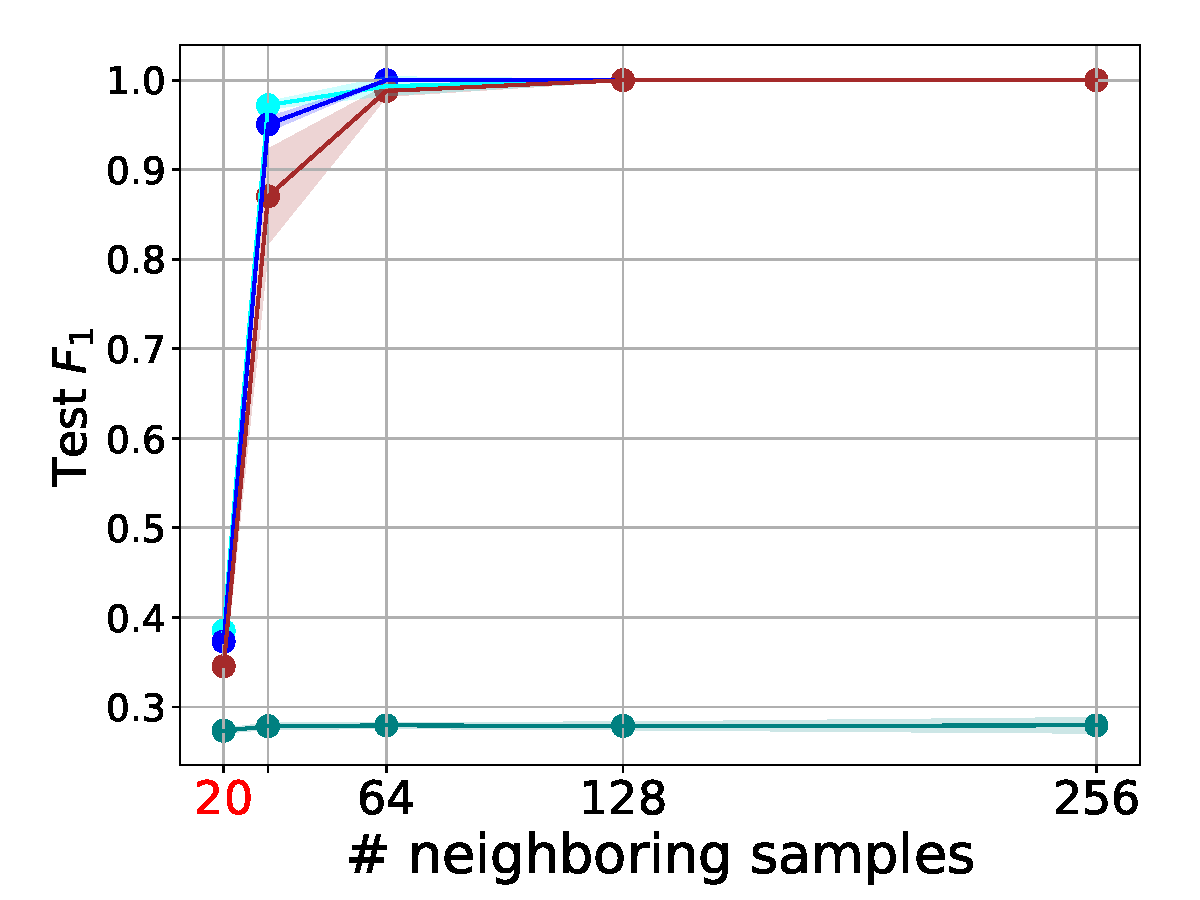
\includegraphics[width=\linewidth]{figs/memory_node/num_neighbors/(64,4000).pdf}
%     \caption{$\causeeffect{64}$}
%     \label{fig:cause_effect_64_num_nei}
%     \end{subfigure}
%     \begin{subfigure}[b]{0.255\textwidth}
%     \centering
%     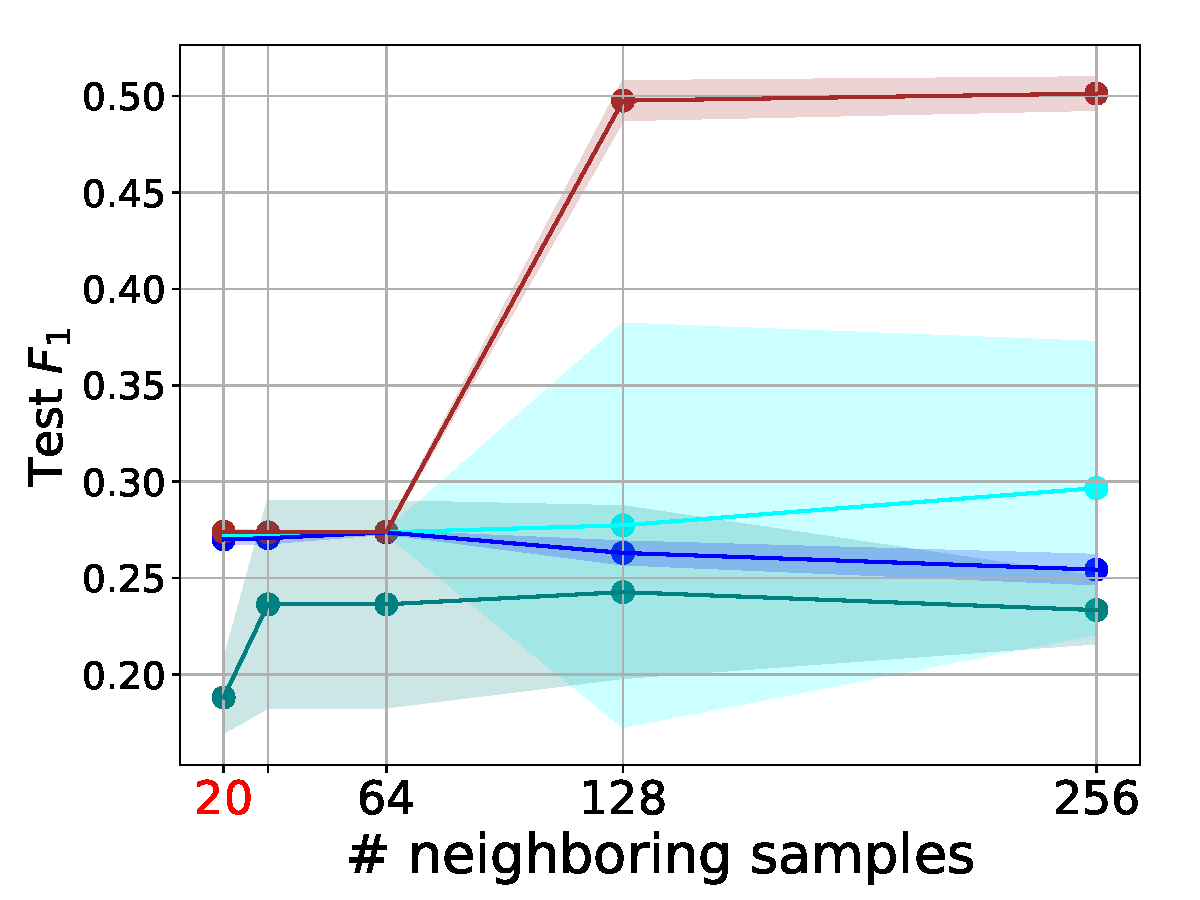
\includegraphics[width=\linewidth]{figs/memory_node/num_neighbors/(256,4000).pdf}
%     \caption{$\causeeffect{256}$}
%     \label{fig:cause_effect_256_num_nei}
%     \end{subfigure}
%     \begin{subfigure}[b]{0.24\textwidth}
%         \centering
%         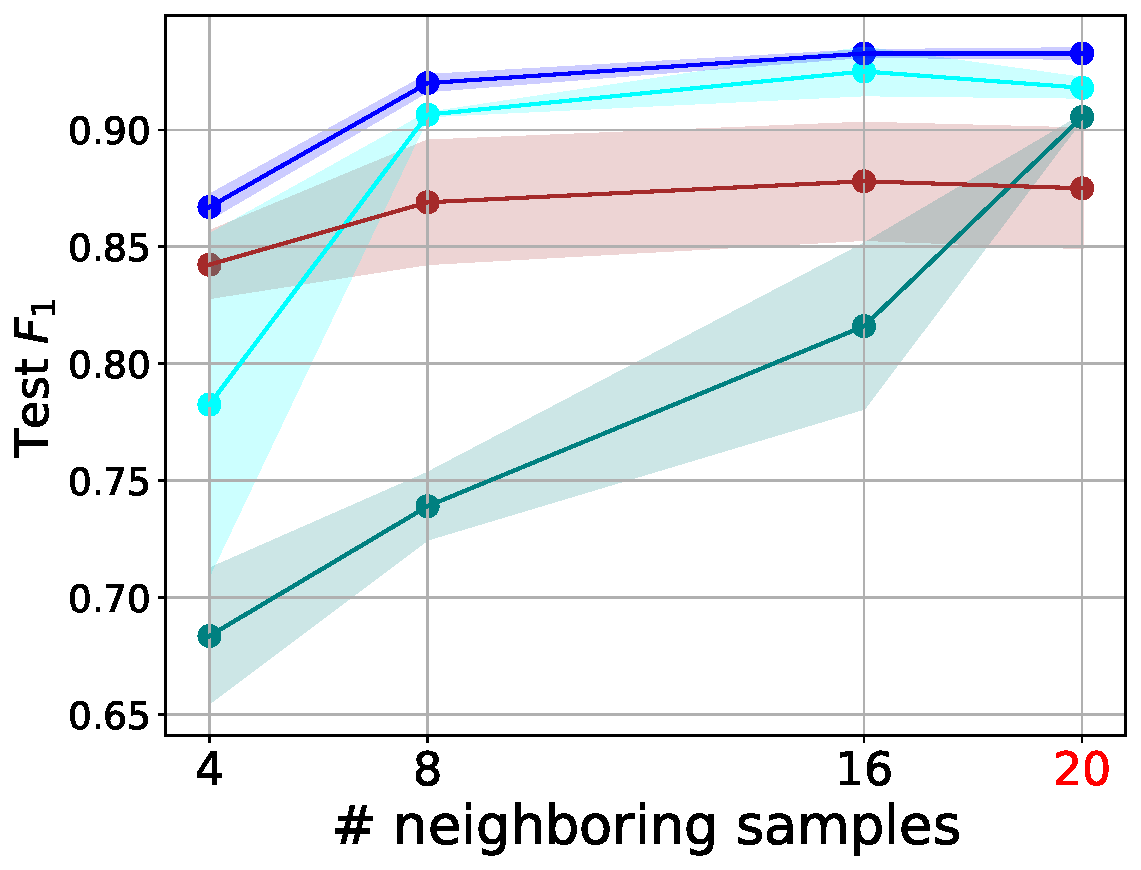
\includegraphics[width=\linewidth]{figs/periodicity/sbm_sto/V2/num_neighboring/multi_seed/(8,1)(0.9, 0.01).pdf}
%         \caption{$\Psto{8, 1}$}
%         \label{fig:sto_periodic_8_num_nei}
%     \end{subfigure}
%     \hfill
%     \begin{subfigure}[b]{0.23\textwidth}
%         \centering
%         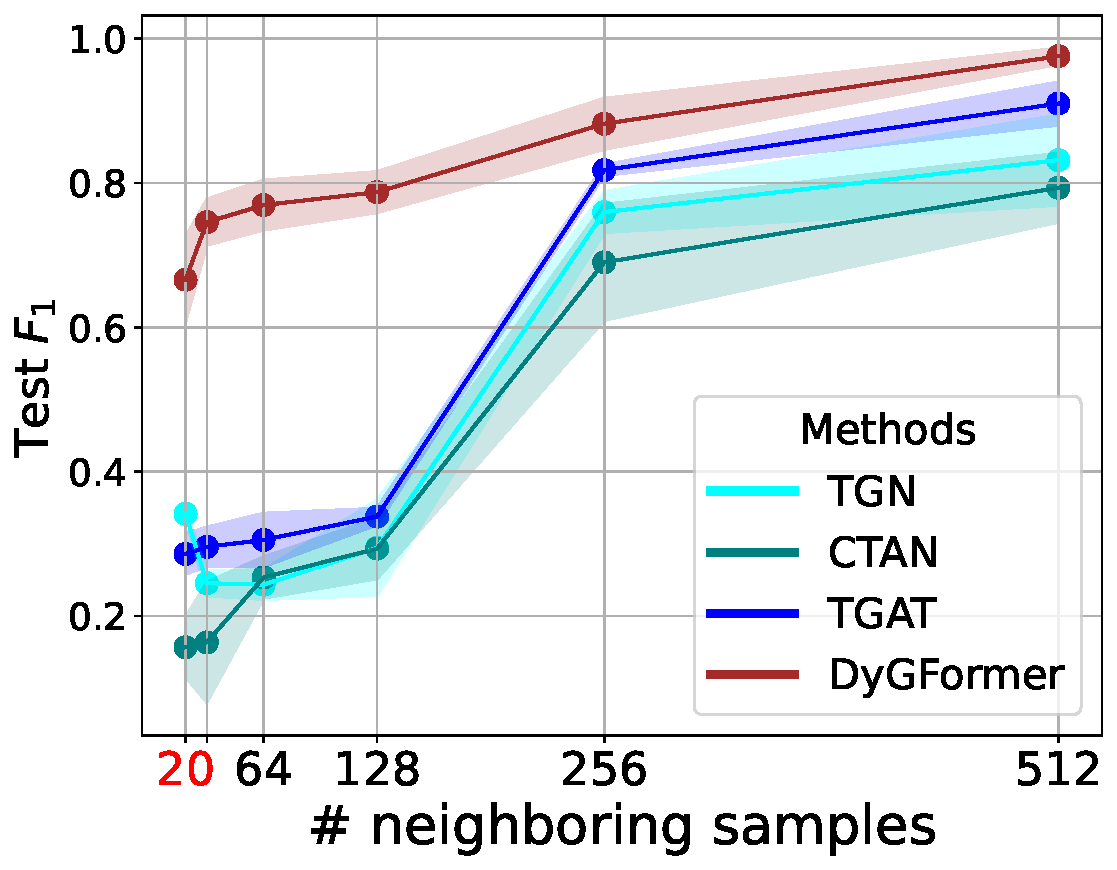
\includegraphics[width=\linewidth]{figs/periodicity/Fixed_ER/num_neighboring/multi_seed/(256,1).pdf}
%         \caption{$\Pdet{256, 1}$}
%         \label{fig:det_periodic_256_num_nei}
%         \label{fig:sub_all_(k, 1)_(0.9, 0.01)_sbm_sto}
%     \end{subfigure}
    
%     \caption{Impact of the number of neighboring samples on cause-and-effect and periodic tasks.}
%     \label{fig:multi_seed_neighbors}
% \end{figure}


\begin{figure}[t]
    % (k, 1) CTDG
    \centering
    \begin{subfigure}[b]{0.24\textwidth}
        \centering
        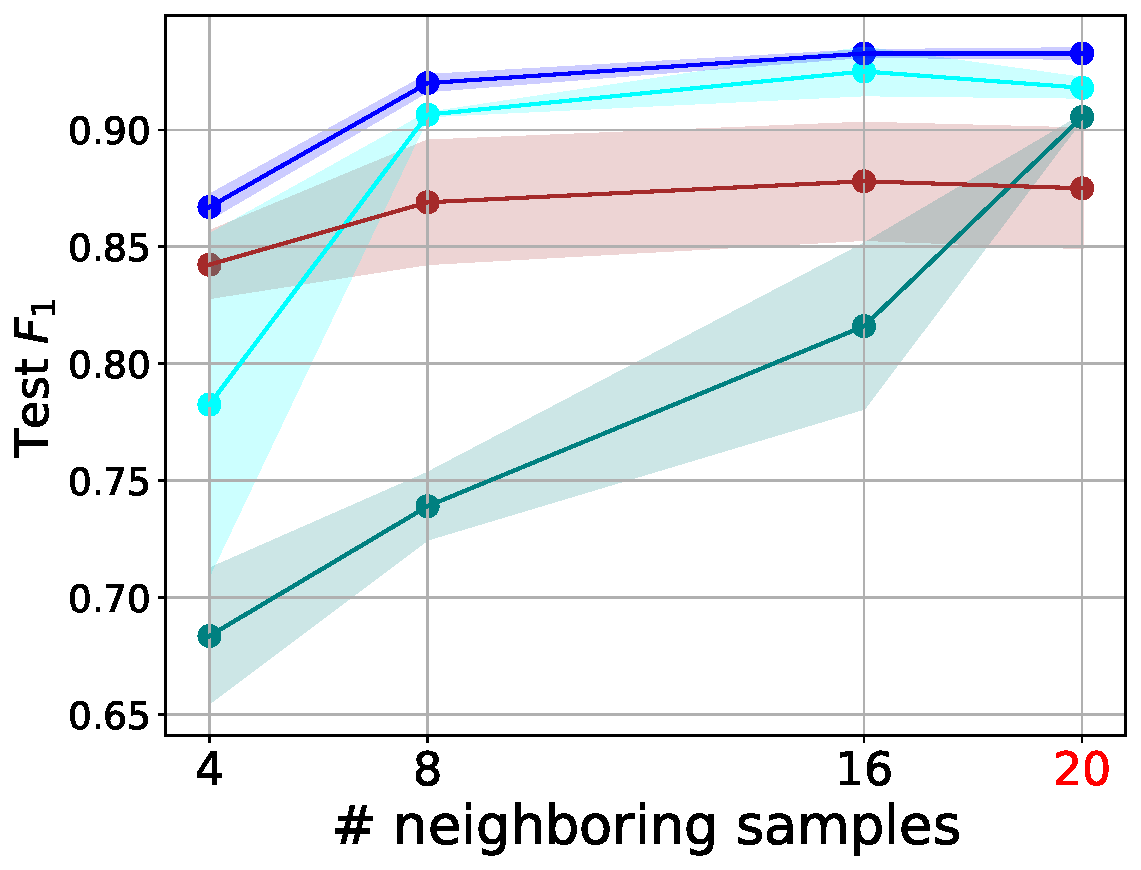
\includegraphics[width=\linewidth]{figs/periodicity/sbm_sto/V2/num_neighboring/multi_seed/(8,1)(0.9, 0.01).pdf}
        \caption{$\Psto{8, 1}$}
        \label{fig:sto_periodic_8_num_nei}
    \end{subfigure}
    \hfill
    \begin{subfigure}[b]{0.232\textwidth}
        \centering
        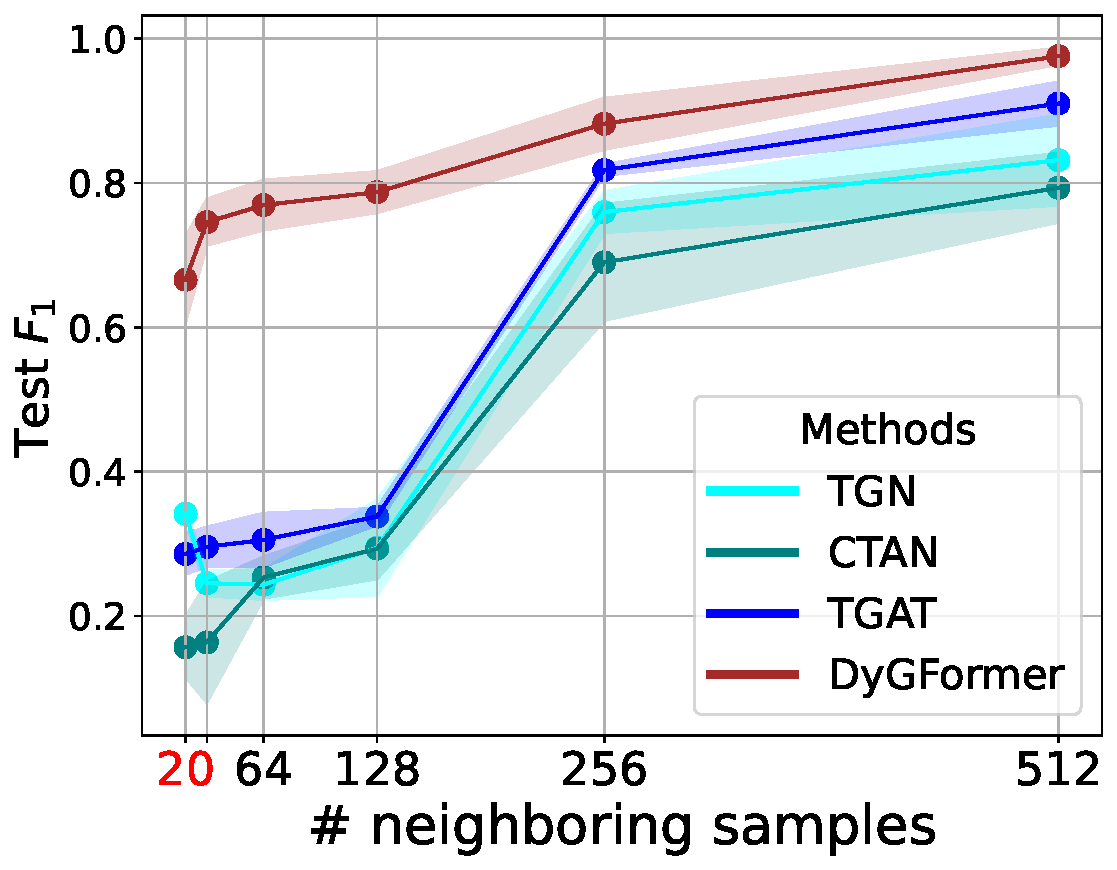
\includegraphics[width=\linewidth]{figs/periodicity/Fixed_ER/num_neighboring/multi_seed/(256,1).pdf}
        \caption{$\Pdet{256, 1}$}
        \label{fig:det_periodic_256_num_nei}
        \label{fig:sub_all_(k, 1)_(0.9, 0.01)_sbm_sto}
    \end{subfigure}
    \hfill
    \begin{subfigure}[b]{0.25\textwidth}
    \centering
    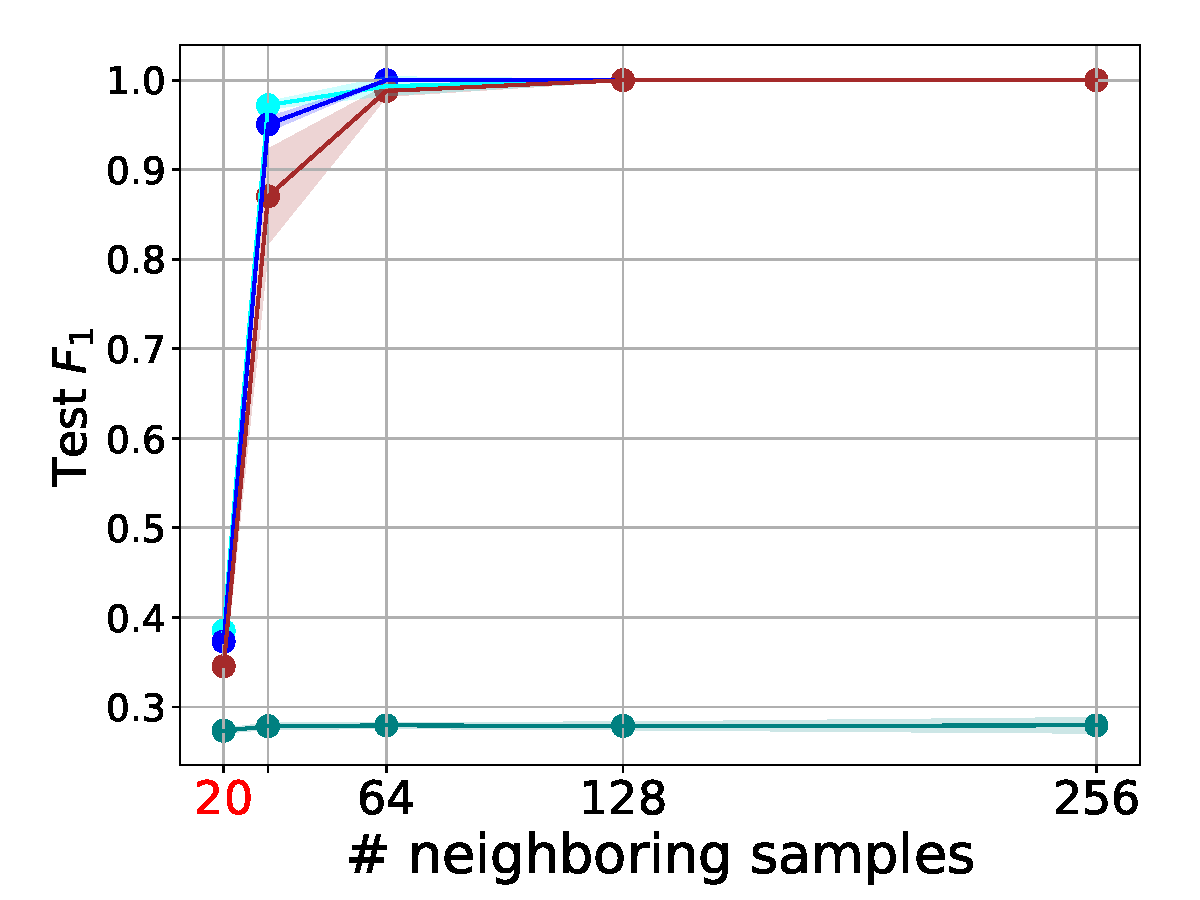
\includegraphics[width=\linewidth]{figs/memory_node/num_neighbors/(64,4000).pdf}
    \caption{$\causeeffect{64}$}
    \label{fig:cause_effect_64_num_nei}
    \end{subfigure}
    \begin{subfigure}[b]{0.25\textwidth}
    \centering
    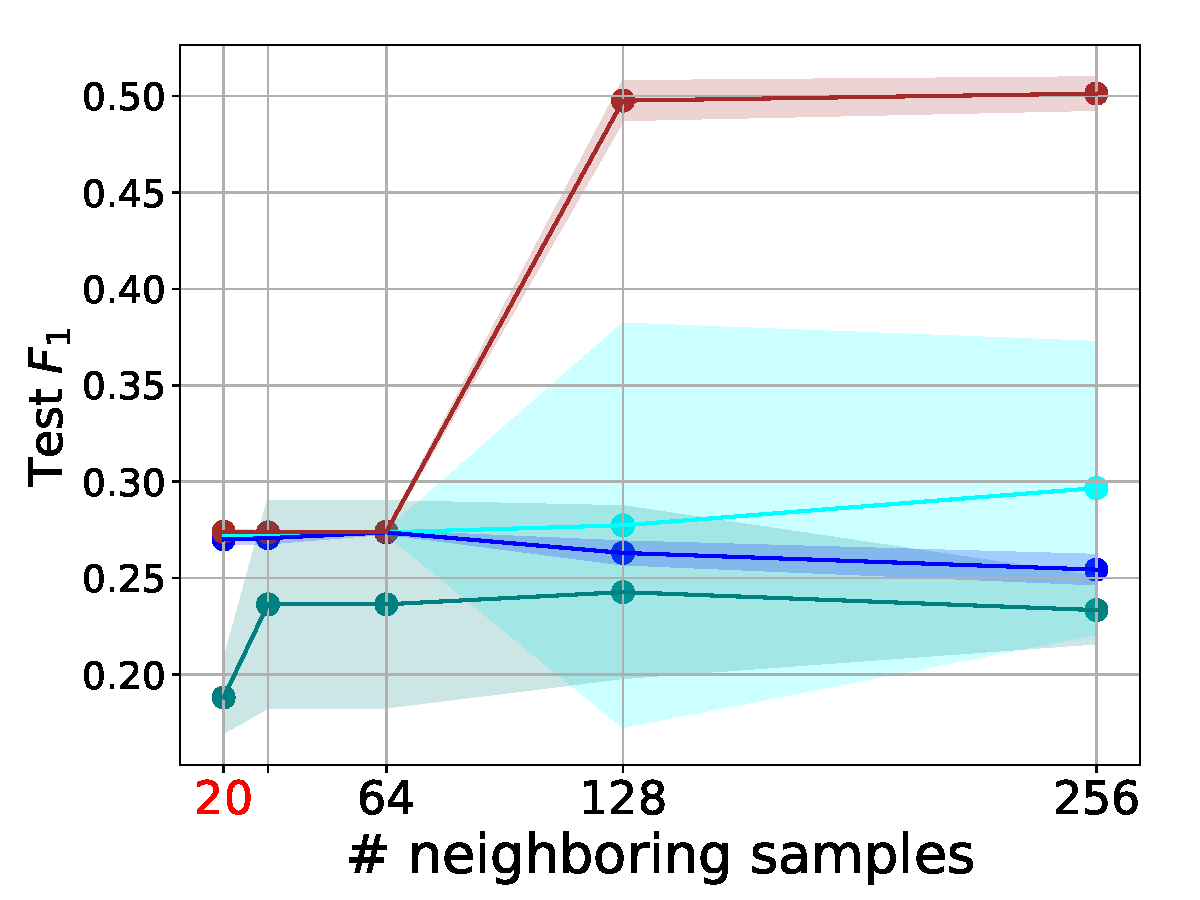
\includegraphics[width=\linewidth]{figs/memory_node/num_neighbors/(256,4000).pdf}
    \caption{$\causeeffect{256}$}
    \label{fig:cause_effect_256_num_nei}
    \end{subfigure}
    
    \caption{Effect of the number of neighbors on periodic (left), and cause-and-effect (right) tasks .}
    \label{fig:multi_seed_neighbors}
\end{figure}



% For further investigation, This motivates us to train TGN with three different number of neighbors, as depicted at Figure~\ref{fig:(K,1)_TGN}: the default 20 ("TGN"), a size equal to the period length ("TGN-K"), and double the period length ("TGN-2K"). Empirically, TGN performs significantly better when using twice the period length, surpassing both the default 20 and the same-size period settings. \\





